\documentclass[a4paper,14pt]{extarticle}

% --- Шрифты и языки ---
\usepackage{fontspec} % поддержка любых шрифтов
\setmainfont{Times New Roman} % основной шрифт
\setmonofont{Courier New} % моноширинный шрифт с кириллицей
\newfontfamily\cyrillicfonttt{Courier New}
\usepackage{polyglossia}
\setmainlanguage{russian}
\setotherlanguage{english}

% --- Основные пакеты ---
\usepackage{graphicx}
\usepackage{caption}
\usepackage{setspace}
\usepackage{indentfirst}
\usepackage{titlesec}
\usepackage[left=30mm, right=15mm, top=20mm, bottom=20mm]{geometry}

% --- Основной текст ---
\setlength{\parindent}{1.25cm} % абзацный отступ
\onehalfspacing% межстрочный интервал

% --- Подписи к рисункам ---
\captionsetup{
	labelsep=period,
	justification=centering,
	font=normalsize
}

% --- Заголовки разделов (1 уровень) ---
\titleformat{\section}
{\bfseries\centering\fontsize{16}{19}\selectfont}
{\thesection}{1em}{}
\titlespacing*{\section}{0pt}{2\baselineskip}{1.5\baselineskip}

% --- Заголовки подразделов (2 уровень) ---
\titleformat{\subsection}
{\bfseries\fontsize{15}{18}\selectfont}
{\thesubsection}{1em}{}
\titlespacing*{\subsection}{0pt}{1.5\baselineskip}{1\baselineskip}

\sloppy


\begin{document}

\begin{titlepage}
    \centering
    {\large Донской Государственный Технический Университет}\\[4cm]

    {\bfseries\LARGE Лабораторные работы №1-15}\\[0.5cm]
    {\large по дисциплине <<Операционные системы>>}\\[6cm]

    \begin{flushright}
        Выполнил: студент группы ВИАС21\\
        Илья Бондаренко
    \end{flushright}

    \vfill

    Ростов-на-Дону --- 2025
\end{titlepage}


\tableofcontents
\newpage

\section{Лабораторная работа №11}

\subsection{Задание №1}
\begin{figure}[h]
	\centering
	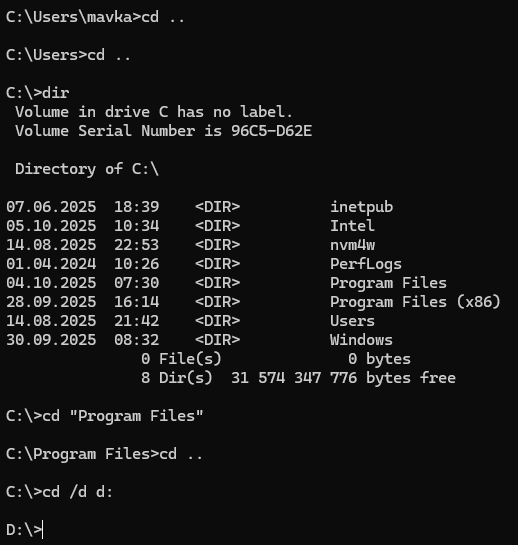
\includegraphics[width=1\textwidth]{./images/11/1_1.png}
\end{figure}
\clearpage

\begin{figure}[h]
	\centering
	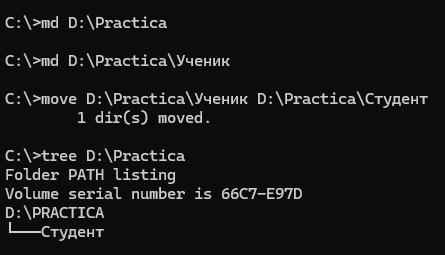
\includegraphics[width=1\textwidth]{./images/11/1_2.png}
\end{figure}

\begin{figure}[h]
	\centering
	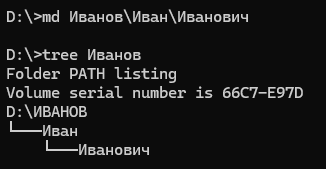
\includegraphics[width=1\textwidth]{./images/11/1_3.png}
\end{figure}
\clearpage

\subsection{Задание №2}
\begin{figure}[h]
	\centering
	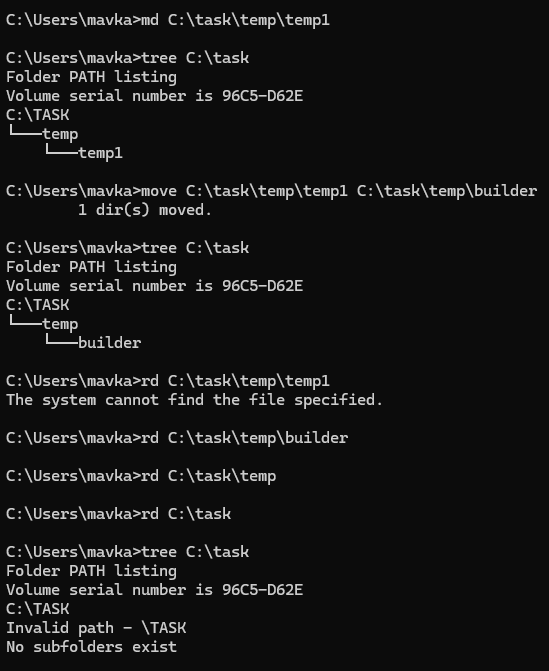
\includegraphics[width=0.9\textwidth]{./images/11/2_1.png}
\end{figure}
\clearpage

\subsection{Задание №3}
\begin{figure}[h]
	\centering
	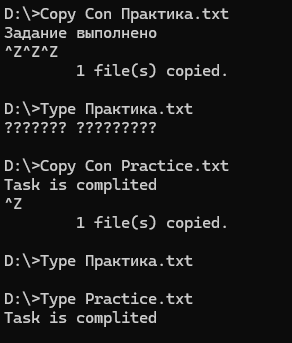
\includegraphics[width=1\textwidth]{./images/11/3_1.png}
\end{figure}
\clearpage

\subsection{Задание №4}
\begin{figure}[h]
	\centering
	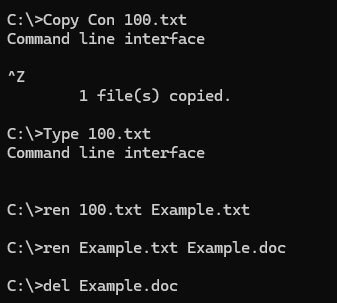
\includegraphics[width=1\textwidth]{./images/11/4_1.png}
\end{figure}
\clearpage

\begin{figure}[h]
	\centering
	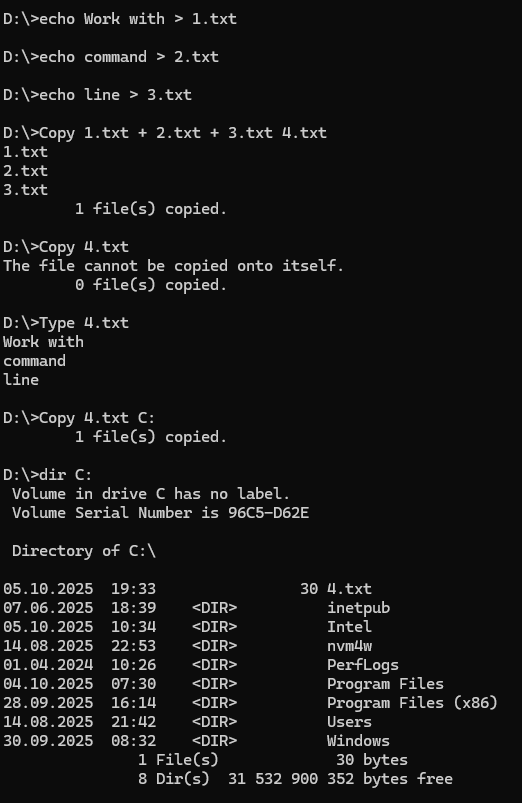
\includegraphics[width=1\textwidth]{./images/11/4_2.png}
\end{figure}
\clearpage

\begin{figure}[h]
	\centering
	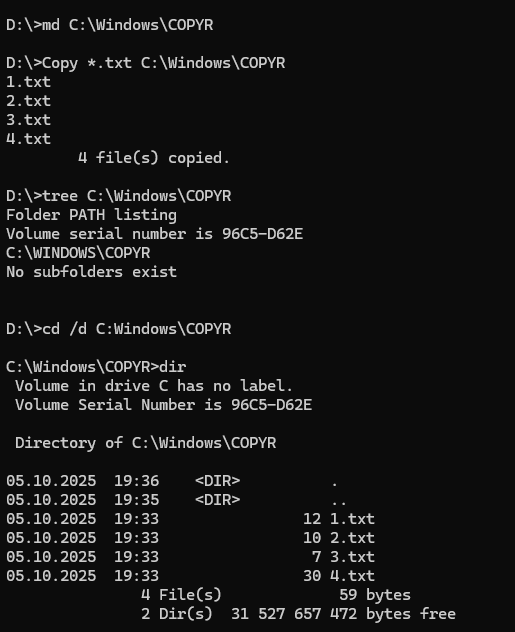
\includegraphics[width=1\textwidth]{./images/11/4_3.png}
\end{figure}
\clearpage

\subsection{Задание №5}
\begin{figure}[h]
	\centering
	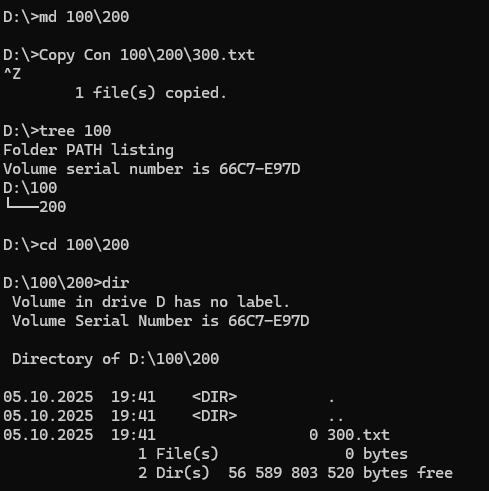
\includegraphics[width=1\textwidth]{./images/11/5_1.png}
\end{figure}
\clearpage

\begin{figure}[h]
	\centering
	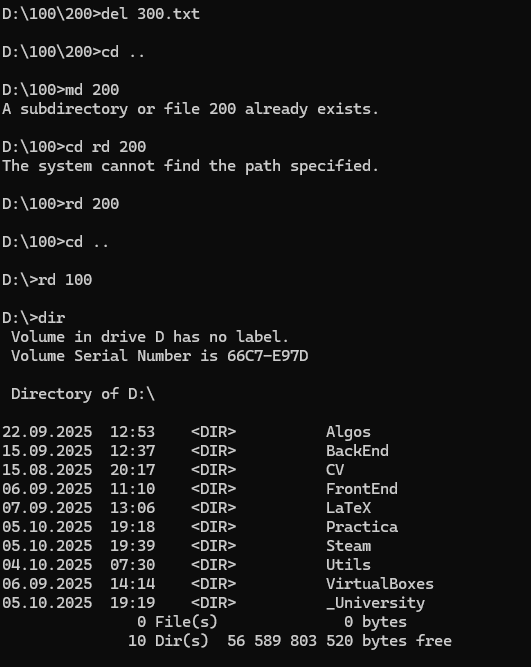
\includegraphics[width=1\textwidth]{./images/11/5_2.png}
\end{figure}
\clearpage

\subsection{Итоговое задание}
\begin{figure}[h]
	\centering
	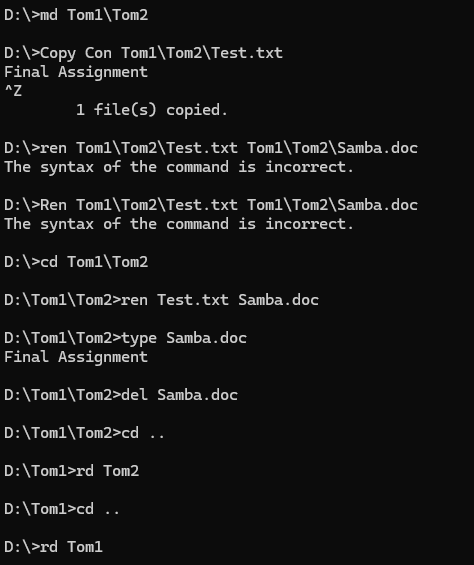
\includegraphics[width=1\textwidth]{./images/11/6_1.png}
\end{figure}
\clearpage

\begin{figure}[h]
	\centering
	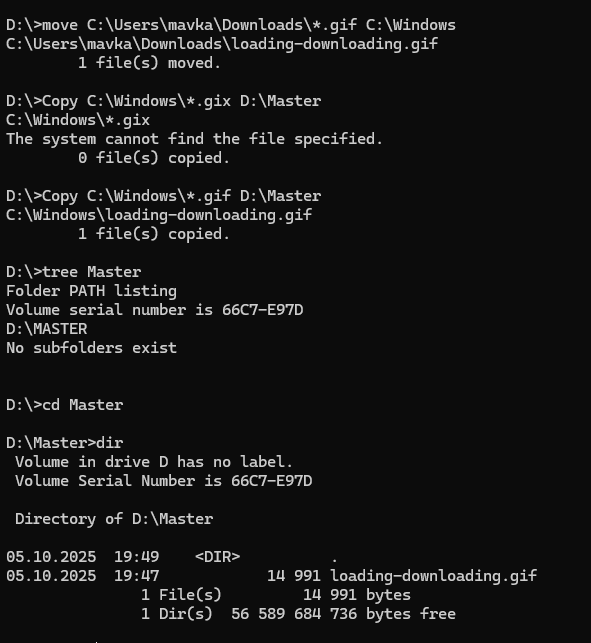
\includegraphics[width=1\textwidth]{./images/11/6_2.png}
\end{figure}
\clearpage

\end{document}